% LaTeX Template for short student reports. Citations should be in bibtex format
% and go in references.bib
\documentclass[a4paper, 11pt]{article}
\usepackage[top=3cm, bottom=3cm, left = 2cm, right = 2cm]{geometry} 
\geometry{a4paper} 
\usepackage[T1]{fontenc}
%\usepackage{textcomp}
\usepackage{graphicx} 
\usepackage{amsmath,amssymb}  
\usepackage{bm}  
\usepackage[pdftex,bookmarks,colorlinks,breaklinks]{hyperref}  
\hypersetup{linkcolor=black,citecolor=black,filecolor=black,urlcolor=black} %
%black links, for printed output
\usepackage{memhfixc} 
\usepackage{pdfsync}  
\usepackage{fancyhdr}
\pagestyle{fancy}
\usepackage[spanish, es-tabla]{babel}
\usepackage{color}
\usepackage{upquote,listings}
\usepackage{pdflscape}
\usepackage{hyperref}
\usepackage{setspace}
\usepackage{parskip}
\usepackage{array}
\usepackage{pdflscape}
\usepackage{caption}
\captionsetup[table]{skip=10pt}


\definecolor{codegreen}{rgb}{0,0.6,0}
\definecolor{codegray}{rgb}{0.5,0.5,0.5}
\definecolor{codepurple}{RGB}{219, 48, 122}
\definecolor{backcolour}{RGB}{242, 242, 242}
\definecolor{bookColor}{cmyk}{0,0,0,0.90}  
\color{bookColor}

\lstset{upquote=true}

\lstdefinestyle{mystyle}{
    backgroundcolor=\color{backcolour},   
    commentstyle=\color{codegreen},
    keywordstyle=\color{codepurple},
    numberstyle=\numberstyle,
    stringstyle=\color{codepurple},
    basicstyle=\footnotesize\ttfamily,
    breakatwhitespace=false,
    breaklines=true,
    captionpos=b,
    keepspaces=true,
    numbers=left,
    numbersep=10pt,
    showspaces=false,
    showstringspaces=false,
    showtabs=false,
}
\lstset{style=mystyle}

\newcommand\numberstyle[1]{%
    \footnotesize
    \color{codegray}%
    \ttfamily
    \ifnum#1<10 0\fi#1 |%
}


\title{ Análisis geo-espacial de datos de gps de trayectorias de Albatros de
Layssan. \\
Proyecto final de fundamentos de Sistemas de Información Geográfica \\
}
\author{Ana Maritza Bello Yáñez \\ Profesora: Dra. Magdalena Saldaña}
%\date{}

\begin{document}
\maketitle
\tableofcontents


\section{Objetivos del proyecto}

Se requiere que proyecto que englobe los siguientes elementos:

$\text{\rlap{$\checkmark$}}\square$ Creación de una base de datos sobre un tema
en concreto.

$\text{\rlap{$\checkmark$}}\square$ Base de datos con al menos dos tablas.

$\text{\rlap{$\checkmark$}}\square$ Representación cartográfica derivada de
algún elemento de la base de datos.

$\text{\rlap{$\checkmark$}}\square$ Aplicar al menos dos elementos de
geo-procesamiento.



\section{Resumen}

Para esta práctica, trabajamos con datos de trayectorias de Albatros de Layssan,
que son una especie de ave marina que actualmente se encuentra amenazada
\footnote{De acuerdo a la NORMA Oficial Mexicana NOM-059-SEMARNAT-2010, aquellas
que podrían llegar a encontrarse en peligro de desaparecer a corto o mediano
plazo, si siguen operando los factores que inciden negativamente en su
viabilidad, al ocasionar el deterioro o modificación de su hábitat o disminuir
directamente el tamaño de sus poblaciones.} y cuyo lugar de anidación es en Isla
Guadalupe.

El albatros de Layssan como ave marina, pasa la mayor parte del tiempo en el mar
(a menudo más del 90\%) y solo toca tierra durante la étapa reproductiva.

En esta practica analizamos sus trayectorias anuales y el área en la que se
desplazan durante su etapa reproductiva. El periódo de reproducción va desde el
1 de diciembre hasta el 30 de julio, y está dividida de la siguiente manera:

\begin{table}[h!]
\caption{Etapas reproductivas del Albatros de Layssan.}
\begin{center}
\begin{tabular}{lcc}
    Etapa & Fecha de inicio & Fecha de término \\
    \hline
    Incubación & 1 de diciembre & 6 de febrero \\
    Empollamiento & 7 de febrero & 20 de febrero \\
    Crianza & 21 de febrero & 30 de julio
\end{tabular}
\end{center}
\end{table}



\section{Introducción}

Los sistemas de información geográfica (SIG), son herramientas que nos permiten
trabajar con diferentes tipos de datos geo-espaciales \footnote{Un dato
geoespacial describe un objeto u evento en la superficie de la tierra. Se
conforma de dos coordenadas terrestres y un valor nominal (carácterística del
objeto o evento en cuestión).}, por ejemplo datos vectoriales y datos ráster.

Los \textit{datos vectoriales} son datos de tipo punto, línea y/o polígono que
representan características como propiedades, ciudades, carreteras, montañas o
cuerpos de agua.

Los \textit{datos ráster} son céldas pixeladas o cuadrículadas que se
identifican seún la fila y la columna. Estos datos crean imágenes más complejas
como fotografías e imágenes de satélite.

Los SIG, además de ayudarnos a visualizar los datos geo-espaciales, nos permiten
hacer análisis con el fin de gestionar acciones, dar acciones a emergencias,
establecer prioridades, comprender tendencias y generar mapas e informes.



\section{Desarrollo}


\subsection{Herramientas utilizadas en el proyecto}

Las herramientas utilizadas en este proyecto son QGIS, PostgreSQL y PostGIS.


\subsection{Datos}

Los datos utilizados en esta pŕactica corresponden a las trayectorias de
albatros de Laysan, registradas mediantes dispositivos GPS y GLS
\footnote{Sistema de posicionamiento global y sensor de localización global
respectivamente, por sus siglas en inglés}, de 47 individuos durante los años
2014 a 2018.

Los GPS se programaron para registrar simultáneamente la posición y la velocidad
del albatros cada 20 minutos, lo que permitió grabar de forma contínua durante
12 a 15 días en algunos casos y en otros de 60 a 70 días, durante la etapa
reproductiva \cite{hernandez2019ecologia}.

Para conocer los hábitos migratorios y zonas de distribución en temporada no
reproductiva se instalaron los dispositivos GLS, los cuales fueron recuperados
por lo menos un año después de su instalación.

Los datos crudos se encuentran en formato CSV y contienen los siguientes campos
o atributos:

\begin{table}[h!]
\caption{Campos o atributos de los datos crudos de trayectorias de albatros.}
\begin{center}
    \begin{tabular}{ l  m{7cm} }
        \hline
        Atributo & Descripción \\
        \hline
        date & Formato 'yyyy-mm-dd'. Se refiere a la fecha a la cual se registró
        la posición del ave. \\
        \hline
        latitude & Coordenada geográfica de la posición latitudinal del ave. \\
        \hline
        longitude & Coordenada geográfica de la posición longitudinal del ave.
        \\
        \hline
        name & Se refiere al id asociado al individuo de albatros de Laysan.\\
        \hline
    \end{tabular}
\end{center}
\end{table}

\subsection{Identificación del área de anidamiento de la especie}

El albatros de Laysan es una especie que presenta filopatría, esto quiere decir
que generalmente regresa a su colonia natal para reproducirse.

El albatros de Laysan se encuentra principalmente en el Pacífico Central (Islas
del noroeste de Hawai). Sin embargo en 1983, estableció una nueva colonia en
Isla Guadalupe.

Isla Guadalupe es una isla mexicana de origen volcánico, ubicada frente a la
costa de la península de Baja California y tiene una superficie total de
476,971. Está categorizada como Reserva de la Biosfera ha de acuerdo a la
Secretaría de Medio Ambiente y Recursos Naturales y a la Comisión Nacional de
Áreas Naturales Protegidas.

Isla Guadalupe se conforma de una isla principal y tres islotes principales,
Zapato, Morro Prieto y el Toro.

El albatros de Laysan ha establecido sus colonias en la Punta Sur de la Isla
Principal, cuya ubicación se puede observar en la Fig.
(\ref{fig:ubicacionIslaGpe}).

\begin{figure}[h!]
    \includegraphics[scale=0.60]{figures/Isla Guadalupe.pdf}
    \caption{Ubicación del área de estudio}
    \label{fig:ubicacionIslaGpe}
    \centering
\end{figure}

\subsection{Creación de base de datos}

\lstinputlisting[language=SQL,   
framesep=10pt, framextopmargin=10pt] {../src/create_table_albatross.sql}

\begin{figure}[h!]
    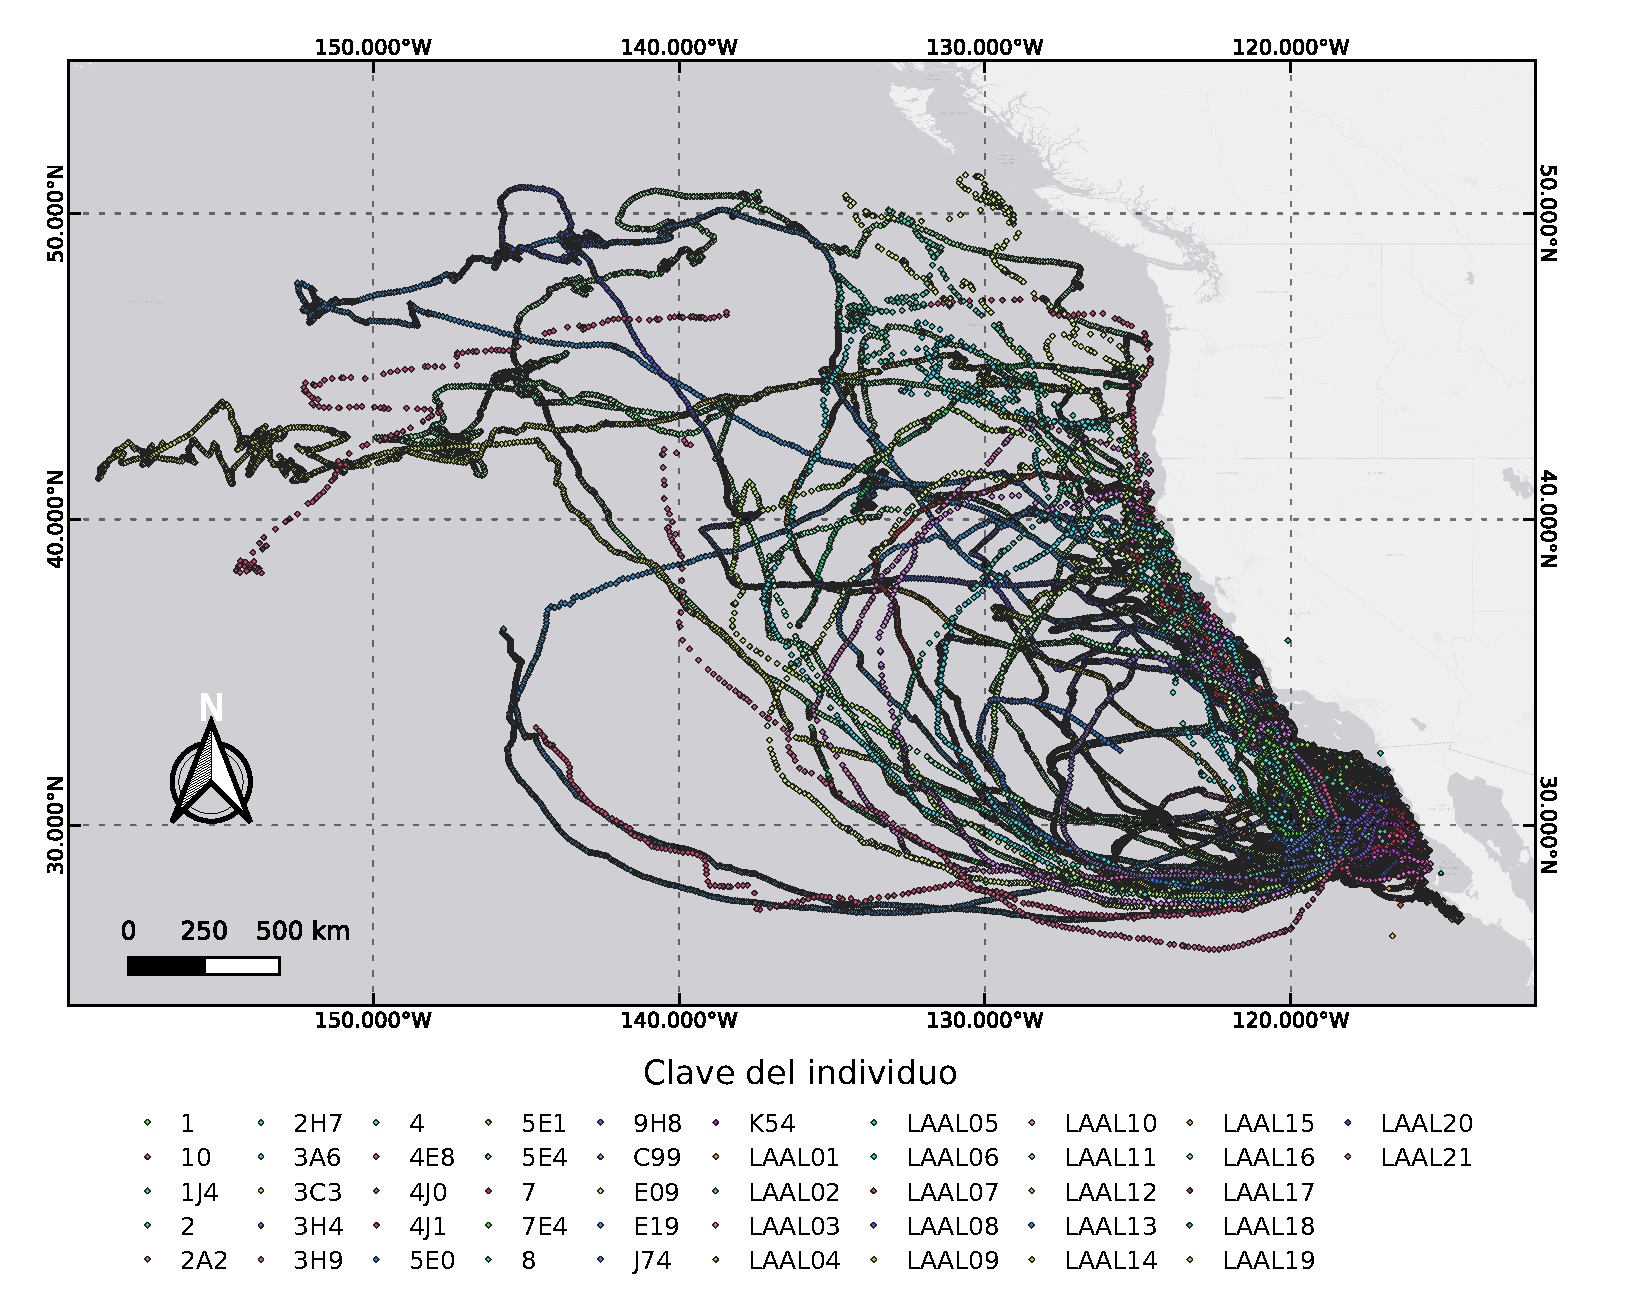
\includegraphics[scale=0.60]{figures/RawData.png}
    \caption{Datos crudos de las trayectorias de albatros}
    \label{fig:trayectorias}
    \centering
\end{figure}


\clearpage
\section{Conclusiones y trabajo a futuro}

\clearpage
\pagebreak
\bibliography{references/references} 
\bibliographystyle{unsrt}

\pagebreak
\section{Anexos}

\lstinputlisting[language=SQL,   
framesep=10pt, framextopmargin=10pt] {../src/create_table_albatross.sql}

\end{document}
